\documentclass[a4paper, 12pt]{article}

\usepackage[brazilian]{babel}
\usepackage[utf8]{inputenc}
\usepackage[T1]{fontenc}
\usepackage[a4paper]{geometry}
\usepackage{amsmath}
\usepackage{amssymb}
\usepackage{indentfirst}
\usepackage{graphicx}
\usepackage[export]{adjustbox}
\usepackage{subcaption}
\renewcommand{\rmdefault}{ptm}

\title{Relatório do EP2}
\author{Beatriz F. Marouelli, \\Leonardo Lana Violin Oliveira}
\date{17 de Maio de 2017}

\begin{document}
\maketitle

\section*{Introdução}
Nosso programa implementa dois métodos de interpolação por partes para funções bivariadas, interpolação bicúbica e interpolação bilinear, para as funções:
$$f(x, y) = x + y$$ 
$$g(x, y) = sen(x - y)$$
$$h(x, y) = (x^2 - y^2)^2$$

\section*{Caso Bilinear}
Definindo 
\begin{align*}
    &h_x = x_{i+1} - x_i &&h_y = y_{i+1} - y_j\\
    &w(x) =\left(\frac{x - x_i}{h_x}\right) &&z(y) = \left(\frac{y - y_j}{h_y}\right)\\
\end{align*}

Inicialemente temos o polinômio interpolador na malha 
$[x_i, x_{i + 1}] \times [y_j, y_{j + 1}]$ na forma matricial:

\[
    s_{ij}^L(x,y) =
\begin{bmatrix}
    1 & w(x) 
\end{bmatrix}
\begin{bmatrix}
    a_{00} & a_{01} \\
    a_{10} & a_{11}
\end{bmatrix}
\begin{bmatrix}
    1 \\
    z(y)
\end{bmatrix}
\]

E as 4 condições de interpolação:
\begin{align}
    s_{ij}^L(x_i,y_j) &= f(x_i, y_j) \tag{1}\\
    s_{ij}^L(x_i,y_{j + 1}) &= f(x_i, y_{j + 1}) \tag{2} \\
    s_{ij}^L(x_{i + 1},y_j) &= f(x_{i + 1}, y_j) \tag{3} \\
    s_{ij}^L(x_{i + 1},y_{j + 1}) &= f(x_{i + 1}, y_{j + 1}) \tag{4}
\end{align}

Expandindo a forma matricial, obtemos:
$$s_{ij}^L(x,y) = a_{00} + a_{10}w(x) + a_{01}z(y) + a_{11}w(x)z(y)$$

Usando a condição $(1)$, temos:
\begin{flalign*}
    f(x_i, y_j) &= a_{00} + a_{10}w(x_i) + a_{01}z(y_j) + a_{11}w(x_i)z(y_j) \\ 
      a_{00} &= f(x_i, y_j)
\end{flalign*}

Usando a condição $(2)$, temos:
\begin{flalign*}
    f(x_i, y_{j+1}) &= a_{00} + a_{10}w(x_i) + a_{01}z(y_{j+1}) + a_{11}w(x_i)z(y_{j+1}) \\
    f(x_i, y_{j+1}) &= a_{00} + a_{01} \\
    a_{01} &= f(x_i, y_{j + 1}) - f(x_i, y_j)
\end{flalign*}

Usando a condição $(3)$, temos:
\begin{flalign*}
    f(x_{i+1}, y_j) &= a_{00} + a_{10}w(x_{i+1}) + a_{01}z(y_j) + a_{11}w(x_{i+1})z(y_j) \\
    f(x_{i+1}, y_j) &= a_{00} + a_{10} \\
    \text{Substituindo $a_{00}$ e isolando $a_{10}$}\\
    a_{10} &= f(x_{i + 1}, y_j) - f(x_i, y_j) 
\end{flalign*}

Usando a condição $(4)$, temos:
\begin{flalign*}
    f(x_{i+1}, y_{j+1}) &= a_{00} + a_{10}w(x_{i+1}) + a_{01}z(y_{j+1}) + a_{11}w(x_{i+1})z(y_{j + 1}) \\
    f(x_{i+1}, y_{j+1}) &= a_{00} + a_{10} + a_{01} + a_{11}\\
    \text{Substituindo $a_{00}$, $a_{10}$ e $a_{01}$}\\
    f(x_{i+1}, y_{j+1}) &= f(x_i, y_j) + f(x_{i+1}, y_j) - f(x_i, y_j) + f(x_i, y_{j+1}) - f(x_i,y_j) + a_{11} \\
    f(x_{i+1}, y_{j+1}) &= -f(x_i, y_j) + f(x_{i+1}, y_j) + f(x_i, y_{j+1}) + a_{11} \\
    \text{Isolando $a_{11}$}\\
    a_{11} &= f(x_{i+1}, y_{j+1}) + f(x_i, y_j) - f(x_{i+1}, y_j) - f(x_i, y_{j+1})
\end{flalign*}

Então ao final da construção, temos o sistema:
\begin{equation*}
    \begin{cases}
        a_{00} = f(x_{i}, y_{j}) \\
        a_{01} = f(x_{i}, y_{j+1}) - f(x_{i}, y_{j}) \\
        a_{10} = f(x_{i+1}, y_{j}) - f(x_{i}, y_{j}) \\
        a_{11} = f(x_{i+1}, y_{j+1}) + f(x_{i}, y_{j}) - f(x_{i+1}, y_{j}) - f(x_{i}, y_{j+1}) \\
    \end{cases}
\end{equation*}

\section*{Caso Bicúbico}
Usando as mesmas definições para $w(x)$, $z(y)$, $h_x$ e $h_y$ que na seção
anterior. Adicionando as derivadas de $w{(x)}$, $w{(x)}^2$, $w{(x)}^3$, $z{(y)}$,
$z{(y)}^2$, $z{(y)}^3$:
\begin{align*}
    &\frac{dw}{dx} = \frac{1}{h_x} \ &\frac{dz}{dy} = \frac{1}{h_y}\\
    &\frac{dw^2}{dx} = \frac{2{(x - x_i)}}{h_{x}^{2}} \ &\frac{dz^2}{dy} = \frac{2{(y-y_j)}}{h_y^2}\\
    &\frac{dw^3}{dx} = \frac{3{(x - x_{i})}^{2}}{h_{x}^{3}} \ &\frac{dz^3}{dy} = \frac{3{(y-y_{j})}^{2}}{h_y^{3}}\\
\end{align*}

Neste caso, a função $s_{ij}^C(x,y)$ na malha $[x_i, x_{i+1}] \times [y_j,
y_{j+1}]$ é dada na forma matricial por:

\[
    s_{ij}^C(x,y) =
\begin{bmatrix}
    1 & w{(x)} & w{(x)}^2 & w{(x)}^3
\end{bmatrix}
\begin{bmatrix}
    a_{00} & a_{01} & a_{02} & a_{03}\\
    a_{10} & a_{11} & a_{12} & a_{13}\\
    a_{20} & a_{21} & a_{22} & a_{23}\\
    a_{30} & a_{31} & a_{32} & a_{33}
\end{bmatrix}
\begin{bmatrix}
    1 \\
    z{(y)} \\
    z{(y)}^2 \\
    z{(y)}^3
\end{bmatrix}
\]

Temos as 4 condições de interpolação:
\begin{align}
    s_{ij}^C(x_i,y_j)&=f(x_i, y_j)\tag{1} \\
    s_{ij}^C(x_i,y_{j + 1})&=f(x_i, y_{j + 1})\tag{2}\\
    s_{ij}^C(x_{i + 1},y_j)&=f(x_{i + 1}, y_j)\tag{3}\\
    s_{ij}^C(x_{i + 1},y_{j + 1})&=f(x_{i + 1}, y_{j + 1})\tag{4}
\end{align}

Temos as 8 condições de interpolação nas derivadas parciais de primeira ordem:
\begin{align}
    \partial_{x}s_{ij}^C(x_{i}, y_{j})      &= \partial_{x}f(x_{i}, y_{j}) \tag{5}      \\
    \partial_{x}s_{ij}^C(x_{i}, y_{j+1})    &= \partial_{x}f(x_{i}, y_{j+1}) \tag{6}    \\
    \partial_{x}s_{ij}^C(x_{i+1}, y_{j})    &= \partial_{x}f(x_{i+1}, y_{j}) \tag{7}    \\
    \partial_{x}s_{ij}^C(x_{i+1}, y_{j+1})  &= \partial_{x}f(x_{i+1}, y_{j+1}) \tag{8}  \\
    \partial_{y}s_{ij}^C(x_{i}, y_{j})      &= \partial_{y}f(x_{i}, y_{j}) \tag{9}      \\
    \partial_{y}s_{ij}^C(x_{i}, y_{j+1})    &= \partial_{y}f(x_{i}, y_{j+1}) \tag{10}   \\
    \partial_{y}s_{ij}^C(x_{i+1}, y_{j})    &= \partial_{y}f(x_{i+1}, y_{j}) \tag{11}   \\
    \partial_{y}s_{ij}^C(x_{i+1}, y_{j+1})  &= \partial_{y}f(x_{i+1}, y_{j+1}) \tag{12}
\end{align}

Além disso, temos as últimas 4 condições com as 4 derivadas parciais de segunda
ordem:
\begin{align}
    \partial_{xy}^{2}s_{ij}^C(x_{i}, y_{j})      &= \partial_{xy}^{2}f(x_{i}, y_{j}) \tag{13}      \\
    \partial_{xy}^{2}s_{ij}^C(x_{i}, y_{j+1})    &= \partial_{xy}^{2}f(x_{i}, y_{j+1}) \tag{14}    \\
    \partial_{xy}^{2}s_{ij}^C(x_{i+1}, y_{j})    &= \partial_{xy}^{2}f(x_{i+1}, y_{j}) \tag{15}    \\
    \partial_{xy}^{2}s_{ij}^C(x_{i+1}, y_{j+1})  &= \partial_{xy}^{2}f(x_{i+1}, y_{j+1}) \tag{16}
\end{align}

Expandindo a forma matricial, obtemos:
\begin{align*}
    s_{ij}^C(x,y) =\ &a_{00} + a_{10}w{(x)} + a_{20}w{(x)}^{2} + a_{30}w{(x)}^{3}\ +          \\ 
               &{(a_{01} + a_{11}w{(x)} + a_{21}w{(x)}^{2} + a_{31}w{(x)}^{3})}z{(y)}\ +     \\ 
               &{(a_{02} + a_{12}w{(x)} + a_{22}w{(x)}^{2} + a_{32}w{(x)}^{3})}z{(y)}^{2}\ + \\
               &{(a_{03} + a_{13}w{(x)} + a_{23}w{(x)}^{2} + a_{33}w{(x)}^{3})}z{(y)}^{3}
\end{align*}

Derivando $s_{ij}^C(x,y)$ parcialmente em relação a $x$, temos:
\begin{align*}
    \partial_{x}s_{ij}^C(x, y) =\ &a_{10}\frac{dw}{dx} + a_{20}\frac{dw^2}{dx} + a_{30}\frac{dw^3}{dx}\ +         \\
                            &\left(a_{11}\frac{dw}{dx} + a_{21}\frac{dw^2}{dx} + a_{31}\frac{dw^3}{dx}\right)z\ + \\ 
                            &\left(a_{12}\frac{dw}{dx} + a_{22}\frac{dw^2}{dx} + a_{32}\frac{dw^3}{dx}\right)z^2\ + \\ 
                            &\left(a_{13}\frac{dw}{dx} + a_{23}\frac{dw^2}{dx} + a_{33}\frac{dw^3}{dx}\right)z^3 
\end{align*}

Derivando $s_{ij}^C(x,y)$ parcialmente em relação a $y$, temos:
\begin{align*}
    \partial_{y}s_{ij}^C(x, y) =\ &\left(a_{01} + a_{11}w + a_{21}w^2 + a_{31}w^3\right)\frac{dz}{dy}\ + \\ 
                                  &\left(a_{02} + a_{12}w + a_{22}w^2 + a_{32}w^3\right)\frac{dz^2}{dy}\ + \\ 
                                  &\left(a_{03} + a_{13}w + a_{23}w^2 + a_{33}w^3\right)\frac{dz^3}{dy} 
\end{align*}

Derivando $s_{ij}^C(x,y)$ parcialmente em relação a $x$ e depois em $y$, temos:
\begin{align*}
    \partial_{xy}s_{ij}^C(x, y) =\ &\left(a_{11}\frac{dw}{dx} + a_{21}\frac{dw^2}{dx} + a_{31}\frac{dw^3}{dx}\right)
                            \frac{dz}{dy}\ + \\ 
                            &\left(a_{12}\frac{dw}{dx} + a_{22}\frac{dw^2}{dx} + a_{32}\frac{dw^3}{dx}\right)
                            \frac{dz^2}{dy}\ + \\ 
                            &\left(a_{13}\frac{dw}{dx} + a_{23}\frac{dw^2}{dx} + a_{33}\frac{dw^3}{dx}\right)
                            \frac{dz^3}{dy} 
\end{align*}

Usando as condições $1$,  $5$, $9$ e $13$ de interpolação cúbica, obtemos:
\begin{align}
    a_{00} &= f(x_{i}, y_{j}) \tag{17}\\
    a_{10} &= h_{x} \frac{\partial f}{\partial x}(x_{i}, y_{j}) \tag{18} \\
    a_{01} &= h_{y} \frac{\partial f}{\partial y}(x_i, y_j) \tag{19} \\
    a_{11} &= h_x h_y \frac{\partial^2 f}{\partial x \partial y}(x_i, y_j) \tag{20}
\end{align}

Usando as condições $2$, e $10$ e as equações $17$ e $19$, obtemos o sistema:
\begin{align*}
    \begin{cases}
        a_{00} = f(x_{i}, y_{j}) \\
        a_{01} = h_y \frac{\partial f}{\partial y}(x_i, y_j) \\
        a_{00} + a_{01} + a_{02} + a_{03} = f(x_i, y_{j+1}) \\
        a_{01} + 2a_{02} + 3a_{03} = h_y \frac{\partial f}{\partial y}(x_i, y_{j+1}) 
    \end{cases}
\end{align*}

Resolvendo este sistema, temos que:
\begin{align}
    &a_{02} = 3(f(x_i, y_{j+1}) - f(x_i, y_j)) - 
        h_y \left(2\frac{\partial f}{\partial y}(x_i, y_j) + \frac{\partial f}{\partial y}(x_i,y_{j+1})\right)
    \tag{21} \\
    &a_{03} = 2(f(x_i, y_j) - f(x_i, y_{j+1})) + 
    h_y \left(\frac{\partial f}{\partial y}(x_i, y_j) + \frac{\partial f}{\partial y}(x_i,y_{j+1})\right)
    \tag{22}
\end{align}

Usando as condições $3$ e $7$ e as equações $17$ e $18$, obtemos o sistema:
\begin{align*}
    \begin{cases}
        a_{00} = f(x_{i}, y_{j}) \\
        a_{10} = h_x \frac{\partial f}{\partial y}(x_i, y_j) \\
        a_{00} + a_{10} + a_{20} + a_{30} = f(x_{i+1}, y_j) \\
        a_{10} + 2a_{20} + 3a_{30} = h_x \frac{\partial f}{\partial x}(x_{i+1}, y_j) 
    \end{cases}
\end{align*}

Resolvendo este sistema, temos que:
\begin{align}
    &a_{20} = 3(f(x_{i+1}, y_j) - f(x_i, y_j)) - 
    h_x \left(2\frac{\partial f}{\partial x}(x_i, y_j) + \frac{\partial f}{\partial x}(x_{i+1},y_j)\right)
    \tag{23} \\
    &a_{30} = 2(f(x_i, y_j) - f(x_{i+1}, y_j)) + 
    h_x \left(\frac{\partial f}{\partial x}(x_i, y_j) + \frac{\partial f}{\partial x}(x_{i+1},y_j)\right)
    \tag{24}
\end{align}

Usando as condições $6$ e $14$ e as equações $18$ e $20$, obtemos o sistema:
\begin{align*}
    \begin{cases}
        a_{10} = h_{x} \frac{\partial f}{\partial x}(x_{i}, y_{j}) \\
        a_{11} = h_x h_y \frac{\partial^2 f}{\partial x \partial y}(x_i, y_j) \\
        a_{10} + a_{11} + a_{12} + a_{13} = h_x \frac{\partial f}{\partial x}(x_i, y_{j+1}) \\
        a_{11} + 2a_{12} + 3a_{13} = h_x h_y \frac{\partial^2 f}{\partial x \partial y}(x_i, y_{j+1}) 
    \end{cases}
\end{align*}

Resolvendo este sistema, temos que:
\begin{align}
    &a_{12} = 3h_x\left(\frac{\partial f}{\partial x}(x_i, y_{j+1}) - \frac{\partial f}{\partial x}(x_{i}, y_{j})\right) - 
    h_x h_y \left(2\frac{\partial^2 f}{\partial x \partial y}(x_i, y_j) + \frac{\partial^2 f}{\partial x \partial y}(x_i, y_{j+1}) \right)
    \tag{25} \\
    &a_{13} = 2h_x\left(\frac{\partial f}{\partial x}(x_{i}, y_{j}) - \frac{\partial f}{\partial x}(x_i, y_{j+1})\right) + 
    h_x h_y\left(\frac{\partial^2 f}{\partial x \partial y}(x_i, y_j) + \frac{\partial^2 f}{\partial x \partial y}(x_i, y_{j+1})\right)
    \tag{26}
\end{align}

Usando as condições $11$ e $15$ e as equações $19$ e $20$, obtemos o sistema:
\begin{align*}
    \begin{cases}
        a_{01} = h_{y} \frac{\partial f}{\partial y}(x_i, y_j) \\
        a_{11} = h_x h_y \frac{\partial^2 f}{\partial x \partial y}(x_i, y_j)\\
        a_{01} + a_{11} + a_{21} + a_{31} = h_y \frac{\partial f}{\partial y}(x_{i+1}, y_j)\\
        a_{11} + 2a_{21} + 3a_{31} =  h_x h_y \frac{\partial^2 f}{\partial x \partial y}(x_{i+1}, y_j)
    \end{cases}
\end{align*}

Resolvendo este sistema, temos que:
\begin{align}
    &a_{21} = 3h_y\left(\frac{\partial f}{\partial y}(x_{i+1}, y_j) - \frac{\partial f}{\partial y}(x_{i}, y_{j})\right) - 
    h_x h_y \left(2\frac{\partial^2 f}{\partial x \partial y}(x_i, y_j) + \frac{\partial^2 f}{\partial x \partial y}(x_{i+1}, y_j) \right)
    \tag{27} \\
    &a_{31} = 2h_y\left(\frac{\partial f}{\partial y}(x_{i}, y_{j}) - \frac{\partial f}{\partial y}(x_{i+1}, y_j)\right) + 
    h_x h_y\left(\frac{\partial^2 f}{\partial x \partial y}(x_i, y_j) + \frac{\partial^2 f}{\partial x \partial y}(x_{i+1}, y_j)\right)
    \tag{28}
\end{align}

Usando as condições $4$, $8$, $12$ e $16$, obtemos o sistema:
\begin{align*}
    \begin{cases}
    a_{22} + a_{23} + a_{32} + a_{33} = f(x_{i+1}, y_{j+1}) + f(x_i, y_j) - f(x_{i+1}, y_j) - f(x_i, y_{j+1}) - a_{11} - a_{12} - a_{13} - a_{21} \\
    2a_{22} + 2a_{23} + 3a_{32} + 3a_{33} = h_x\frac{\partial f}{\partial x}(x_{i+1}, y_{j+1}) - a_{10} - a_{11} - a_{12} - a_{13} - 2a_{20} - 2a_{21} - 3a_{30} - 3a_{31} \\
    2a_{22} + 3a_{23} + 2a_{32} + 3a_{33} = h_y\frac{\partial f}{\partial y}(x_{i+1}, y_{j+1}) - a_{01} - a_{11} - a_{21} - a_{31} - 2a_{02} - 2a_{12} - 3a_{03} - 3a_{13} \\
    4a_{22} + 6a_{23} + 6a_{32} + 9a_{33} = h_x h_y \frac{\partial^2 f}{\partial x \partial y}(x_{i+1}, y_{j+1}) - a_{11} - 2a_{21} - 3a_{31} - 2a_{12} - 3a_{13}
    \end{cases}
\end{align*}

Nomeando as equações do sistema como \textit{eq4}, \textit{eq8}, \textit{eq12} e \textit{eq16}, respectivamente em sua ordem de aparição, temos que:
\begin{align*}
    \begin{cases}
    a_{22} = 3eq4 - eq8 - a_{23} \\
    a_{23} = 3eq12 - eq16 - 2(3eq4 - eq8)\\
    a_{32} =  eq8 - 2eq4 - a_{33}\\
    a_{33} = eq16 - 2eq12 - 2(eq8 - 2eq4)
    \end{cases}
\end{align*}

\section*{Funcionalidades do Programa}
\subsection*{interpolate\_points}
    Recebe as coordenadas dos pontos inicial e final da malha, quantos pontos no eixo \textit{x}, equivalente ao número de colunas da matriz que representa a malha, e quantos pontos no eixo \textit{y}, ou seja, o número de linhas da matriz representativa. Retorna uma matriz com dimensões $(n_y + 1) \times 2 \times (n_x + 1)$ que representa a malha, na qual os números na primeira coluna correspondem ao \textit{x}, e da segunda, ao \textit{y}.

\subsection*{grid}
    Cria os eixos necessários para realizar os plottings. Em especial, o eixo $z$ possui duas versões, os valores da função original, e os da função interpoladora.

\subsection*{find\_values}
    Calcula os valores de uma função \textit{f} nos pontos da malha, achados pela função \textit{interpolate\_points}. Retorna uma matriz com dimensões $(n_y + 1) \times 1 \times (n_x + 1)$ com os resultados.
    
\subsection*{constroiv}
    Cria e insere os coeficientes com os valores em acordo com as equações deduzidas no relatório em uma matriz $2 \times 2 \times (n_x*n_y)$. Estes coeficientes são organizados de acordo com o ponto mais à direita e abaixo do quadrado que contém o ponto a ser calculado.
    
\subsection*{avaliav}
    Primeiramente usa o ponto superior direito de todo quadrado na malha pra determinar em qual retângulo da malha o ponto a ser cálculado está contido. Usa os coeficientes achados na função \textit{constroiv}.
    
\section*{Aviso}
    Caso não consiga visualizar os plottings, o \textit{toolkit gnuplot} precisa ser inicializado 
    através do comando: \textit{graphics\_toolkit ("gnuplot")}.
    
\section*{Imagens dos Gráficos}
\begin{figure}[!htp]
\centering
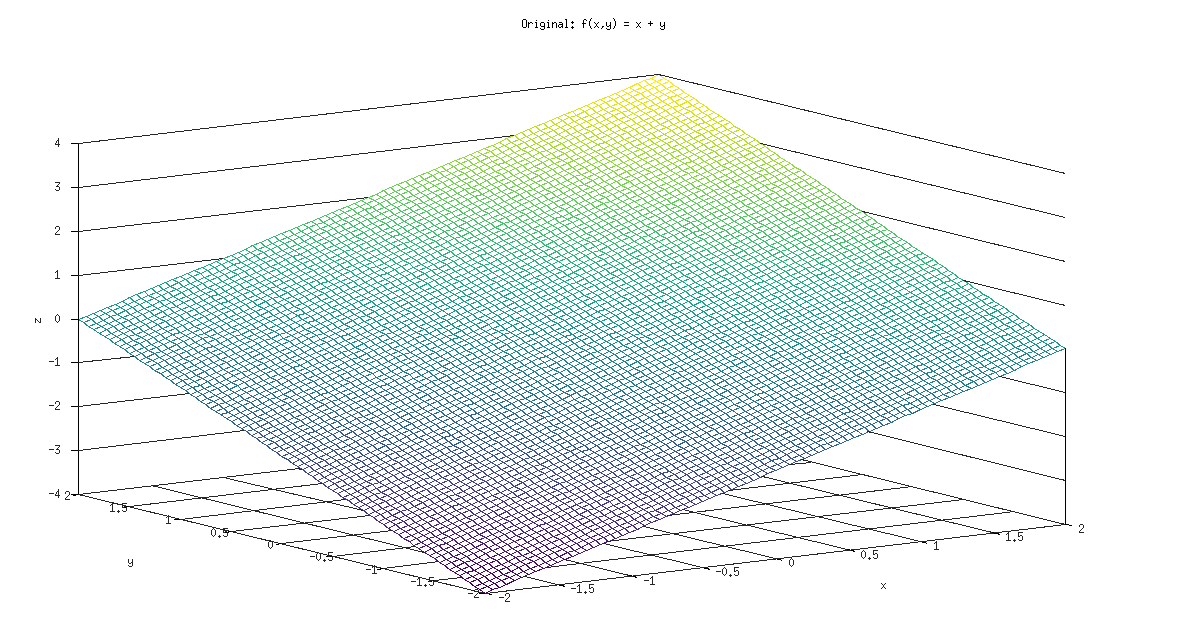
\includegraphics[scale=0.3]{f1.png}
\caption{f(x,y) = x + y}
\end{figure}

\begin{figure}[!htp]
\centering
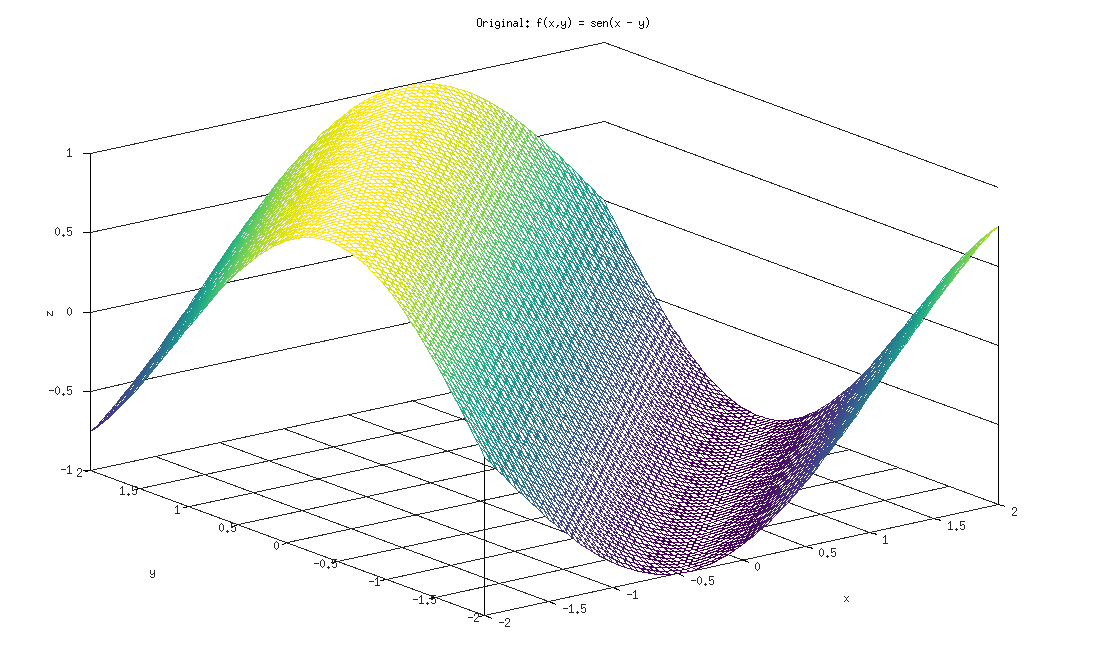
\includegraphics[scale=0.3]{f2.png}
\caption{g(x,y) = sen(x - y)}
\end{figure}

\begin{figure}[!htp]
\centering
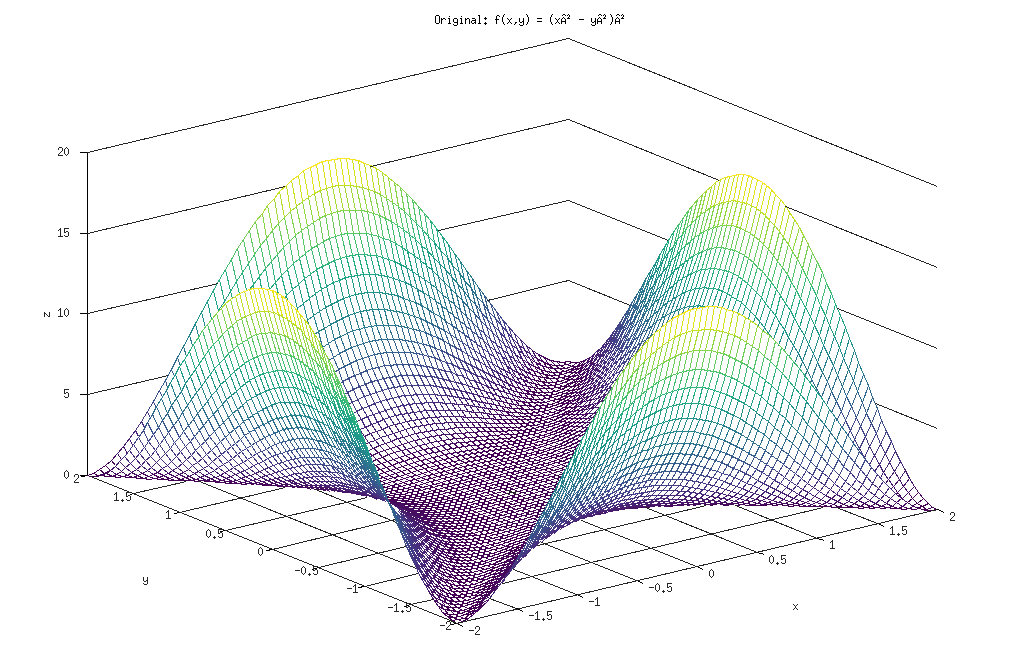
\includegraphics[scale=0.3]{f3.png}
\caption{h(x,y) = $(x^2 - y^2)^2$}
\end{figure}

\begin{figure}[!htp]
\centering
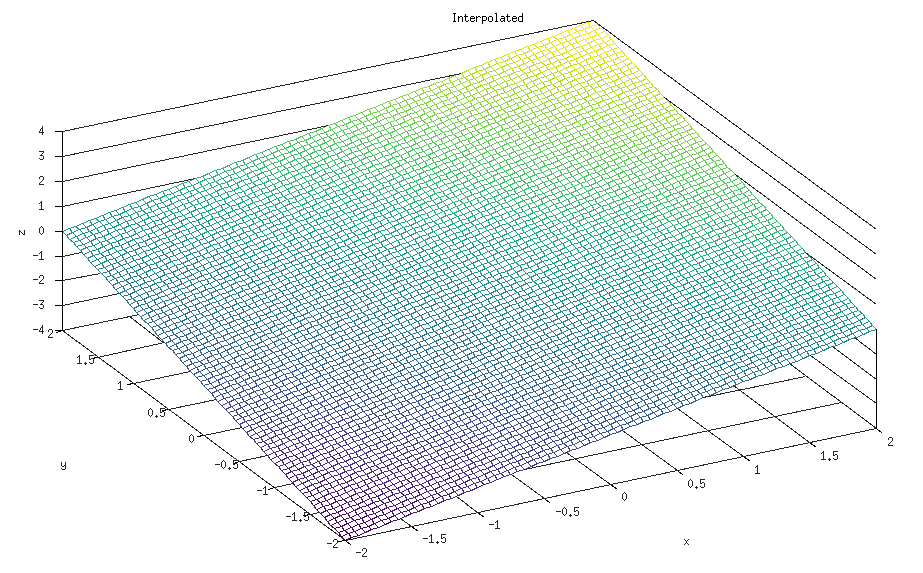
\includegraphics[scale=0.3]{f1_v_bilinear.png}
\caption{Interpolação bilinear de f(x,y)}
\end{figure}

\begin{figure}[!htp]
\centering
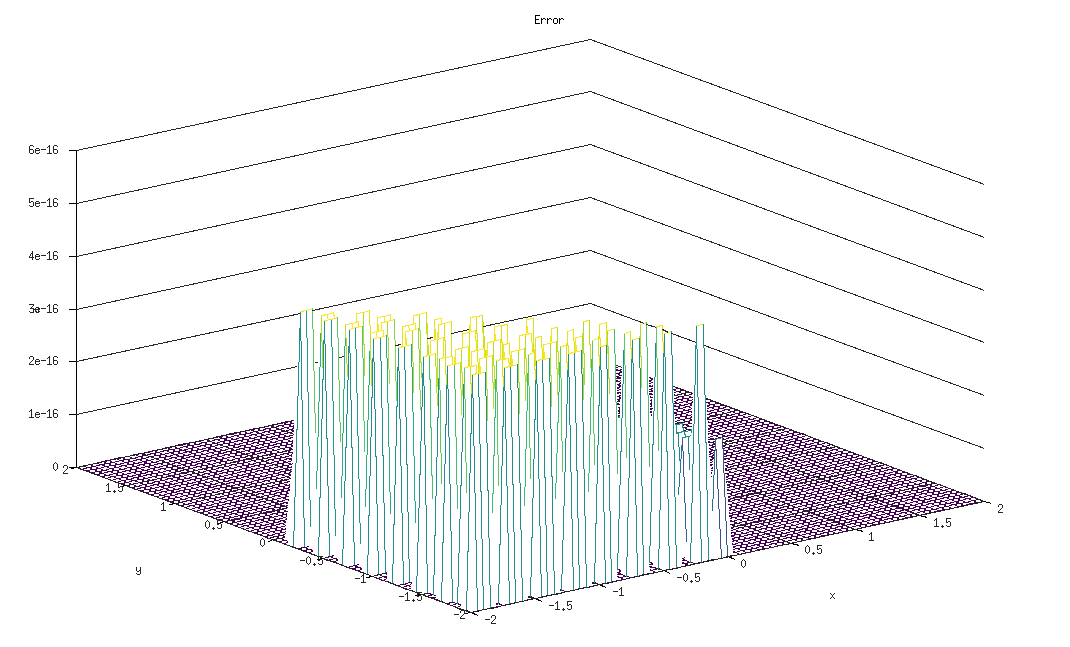
\includegraphics[scale=0.3]{f1_bilinear_error.png}
\caption{Erro da interpolação bilinear de f(x,y)}
\end{figure}

\begin{figure}[!htp]
\centering
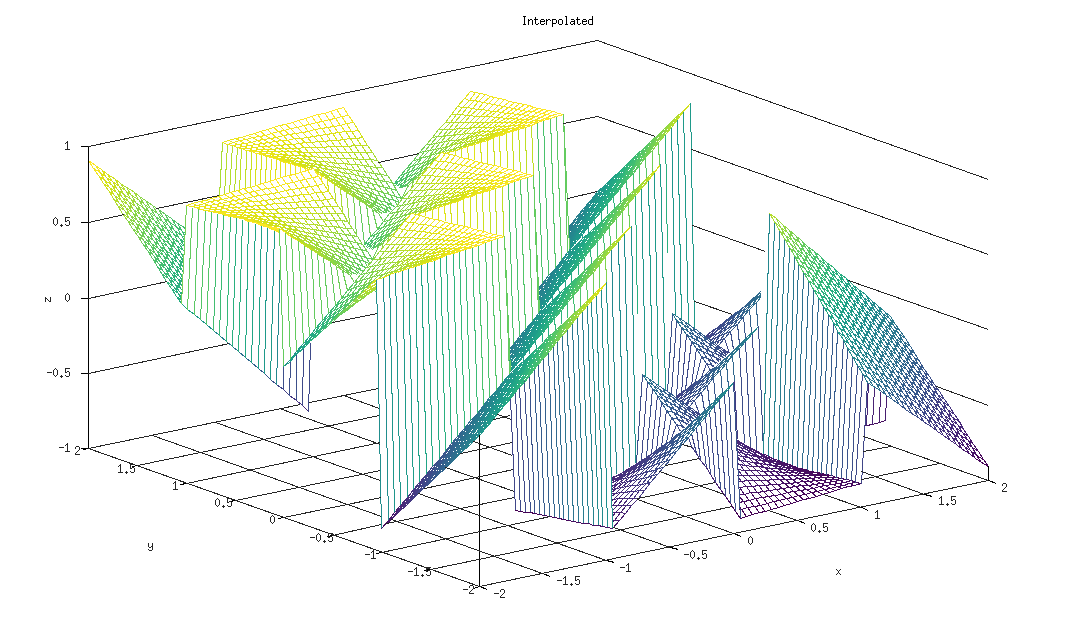
\includegraphics[scale=0.3]{f2_bilinear_v.png}
\caption{Interpolação bilinear de g(x,y)}
\end{figure}

\begin{figure}[!htp]
\centering
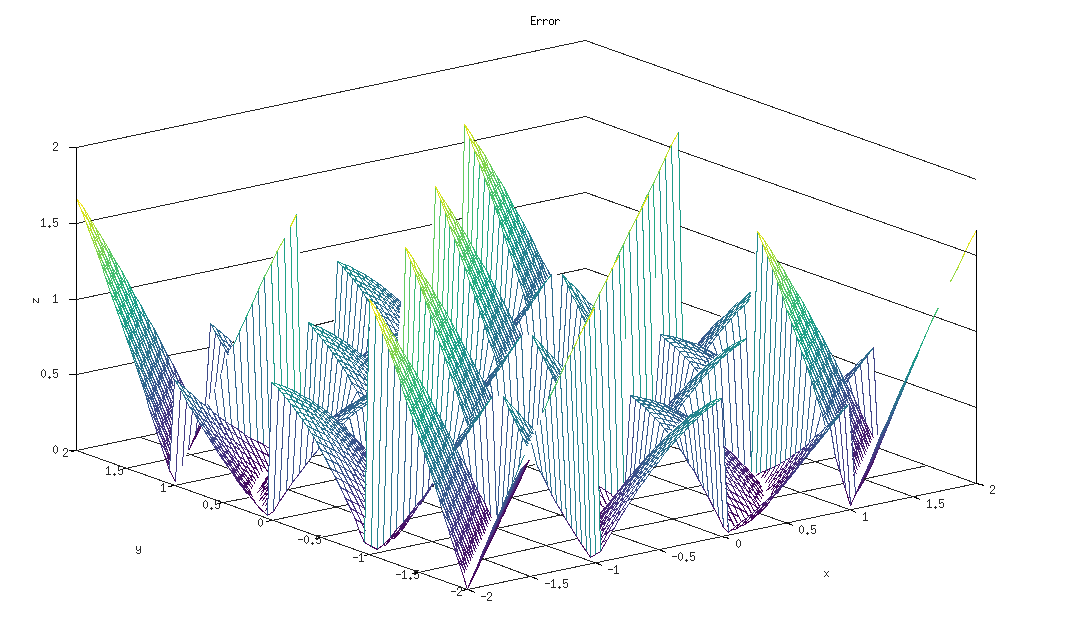
\includegraphics[scale=0.3]{f2_bilinear_error.png}
\caption{Erro da interpolação bilinear de g(x,y)}
\end{figure}

\begin{figure}[!htp]
\centering
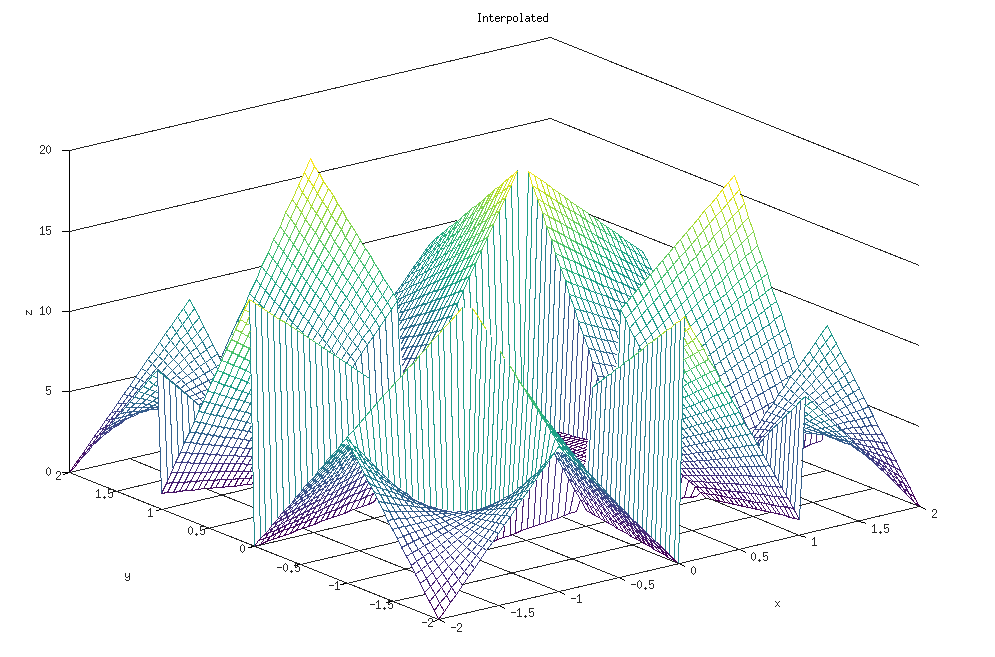
\includegraphics[scale=0.3]{f3_bilinear_v.png}
\caption{Interpolação bilinear de h(x,y)}
\end{figure}

\begin{figure}[!htp]
\centering
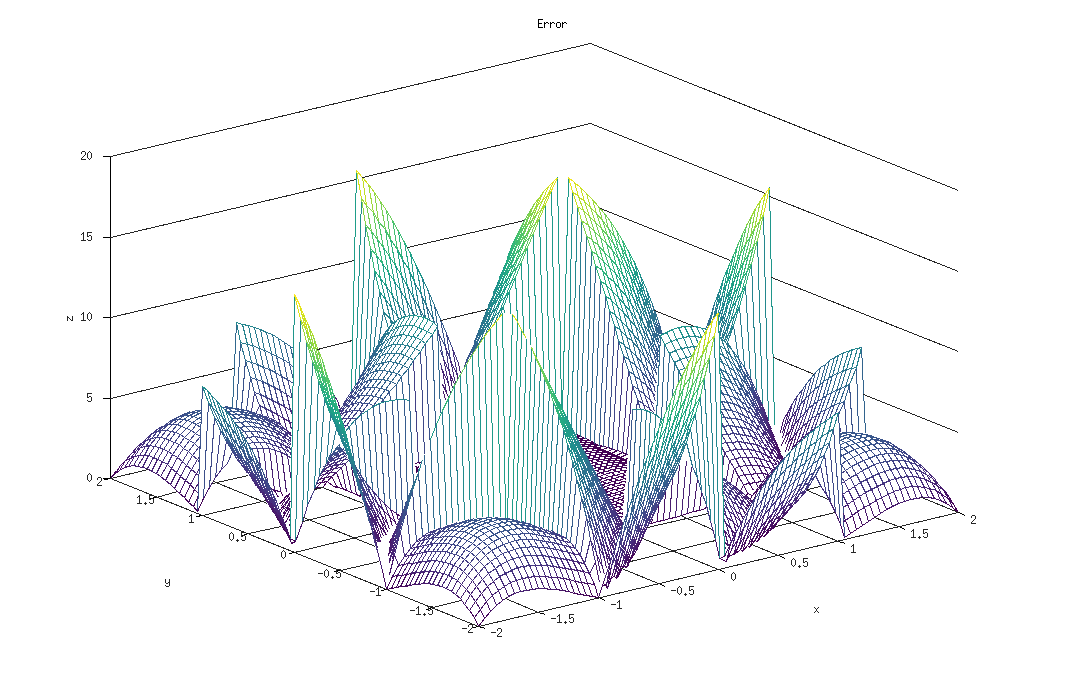
\includegraphics[scale=0.3]{f3_bilinear_error.png}
\caption{Erro da interpolação bilinear de h(x,y)}
\end{figure}

\begin{figure}[!htp]
\centering
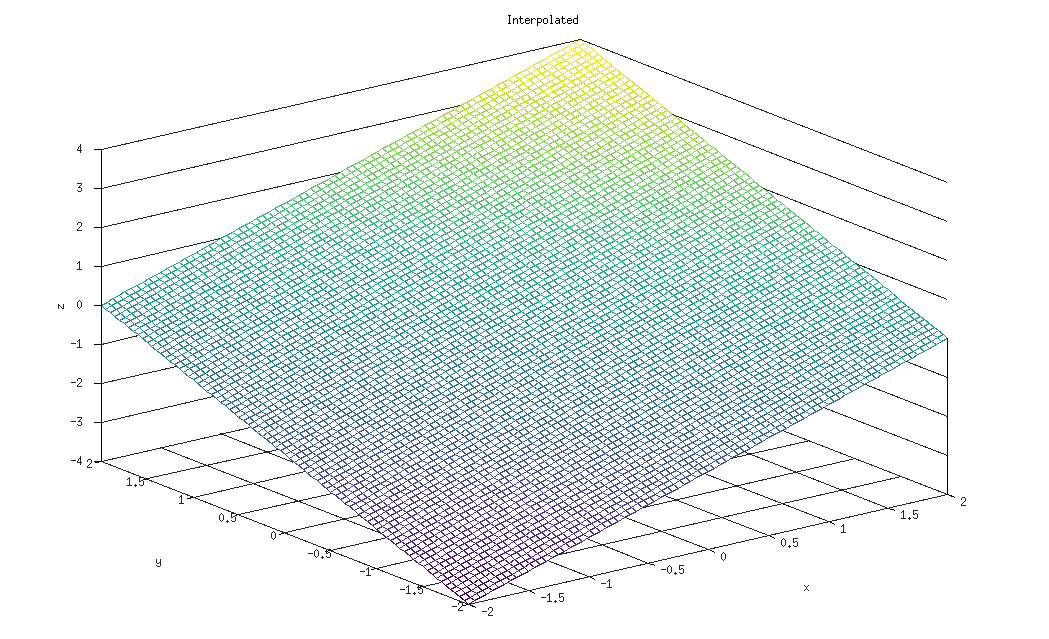
\includegraphics[scale=0.5]{f1_bicubica_v.png}
\caption{Interpolação bicúbica de f(x,y)}
\end{figure}

\begin{figure}[!htp]
\centering
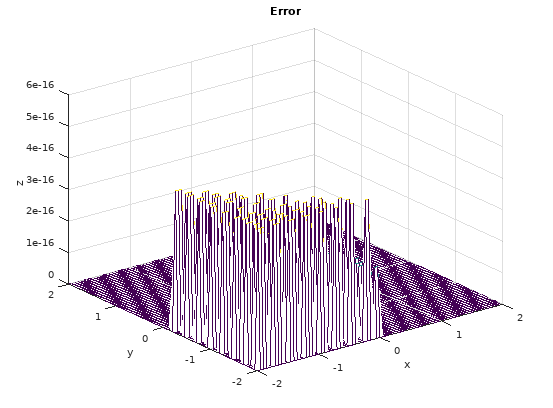
\includegraphics[scale=0.5]{f1_bicubica_error.png}
\caption{Erro da interpolação bicúbica de f(x,y)}
\end{figure}

\begin{figure}[!htp]
\centering
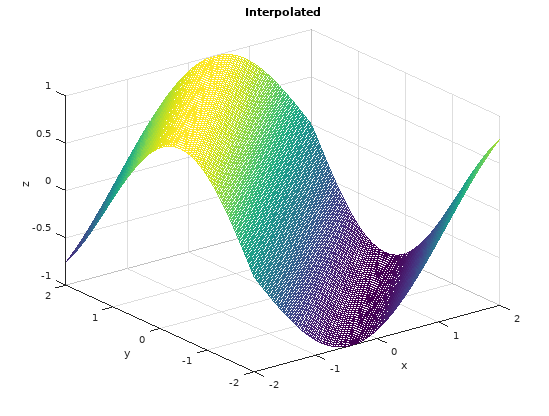
\includegraphics[scale=0.5]{f2_bicubica_v.png}
\caption{Interpolação bicúbica de g(x,y)}
\end{figure}

\begin{figure}[!htp]
\centering
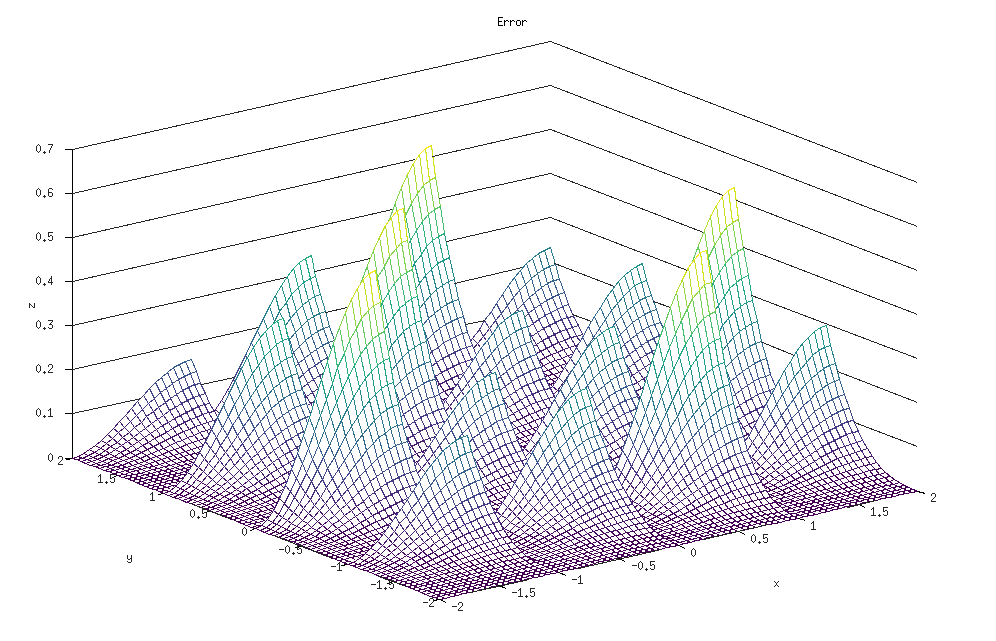
\includegraphics[scale=0.5]{f2_bicubica_error.png}
\caption{Erro da interpolação bicúbica de g(x,y)}
\end{figure}

\begin{figure}[!htp]
\centering
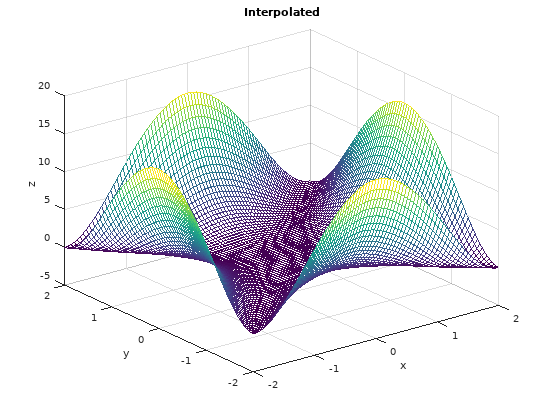
\includegraphics[scale=0.5]{f3_bicubica_v.png}
\caption{Interpolação bicúbica de h(x,y)}
\end{figure}

\begin{figure}[!htp]
\centering
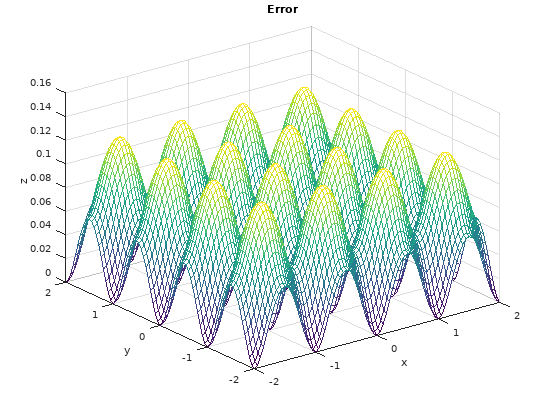
\includegraphics[scale=0.5]{f3_bicubica_error.png}
\caption{Erro da interpolação bicúbica de h(x,y)}
\end{figure}

\begin{figure}[!htp]
\centering
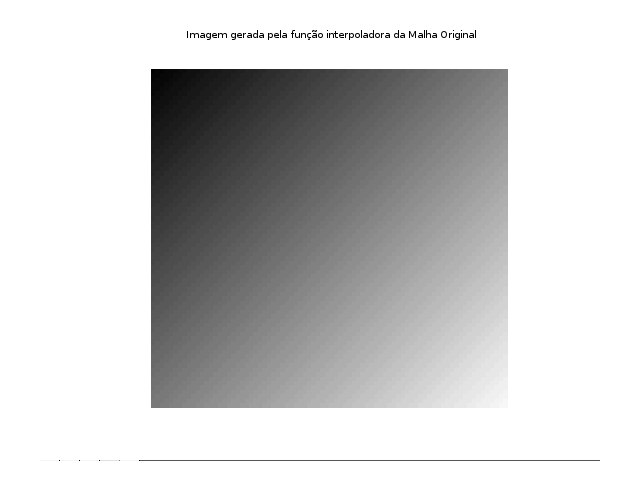
\includegraphics[scale=0.5]{f1_compress_original.png}
\caption{Malha interpolada a partir de f(x,y) com o tamanho original}
\end{figure}

\begin{figure}[!htp]
\centering
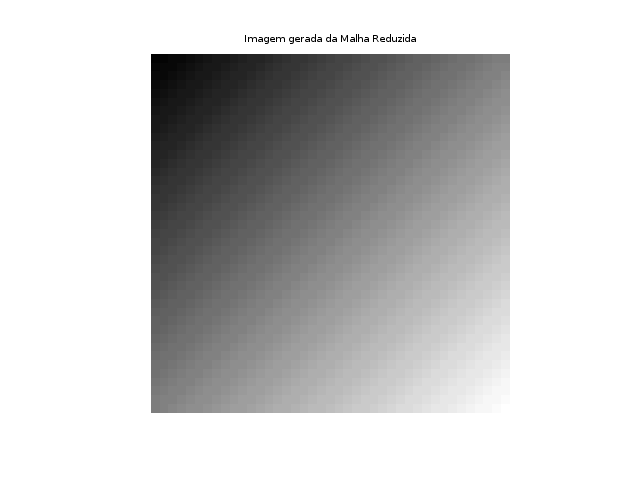
\includegraphics[scale=0.5]{f1_compress_reduced.png}
\caption{Malha interpolada a partir de f(x,y) com o tamanho reduzido}
\end{figure}

\begin{figure}[!htp]
\centering
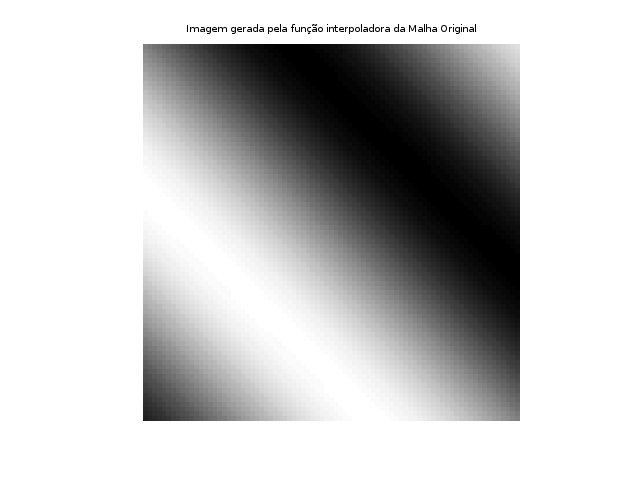
\includegraphics[scale=0.5]{f2_compress_original.png}
\caption{Malha interpolada a partir de g(x,y) com o tamanho original}
\end{figure}

\begin{figure}[!htp]
\centering
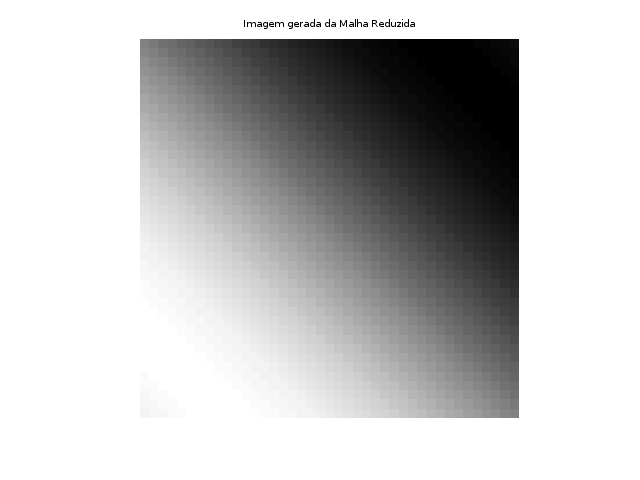
\includegraphics[scale=0.5]{f2_compress_reduced.png}
\caption{Malha interpolada a partir de g(x,y) com o tamanho reduzido}
\end{figure}

\begin{figure}[!htp]
\centering
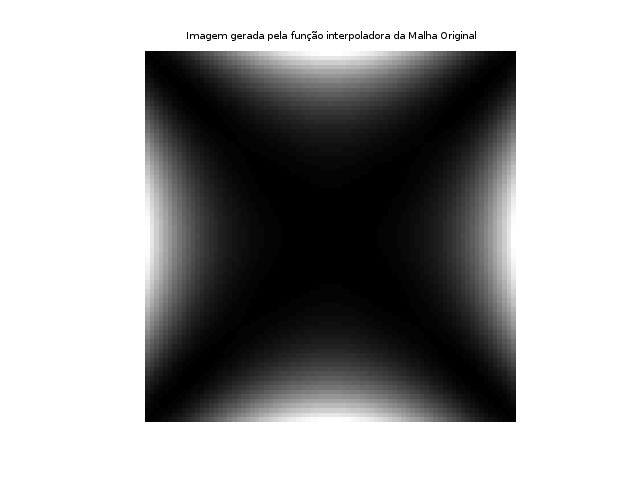
\includegraphics[scale=0.5]{f3_compress_original.png}
\caption{Malha interpolada a partir de h(x,y) com o tamanho original}
\end{figure}

\begin{figure}[!htp]
\centering
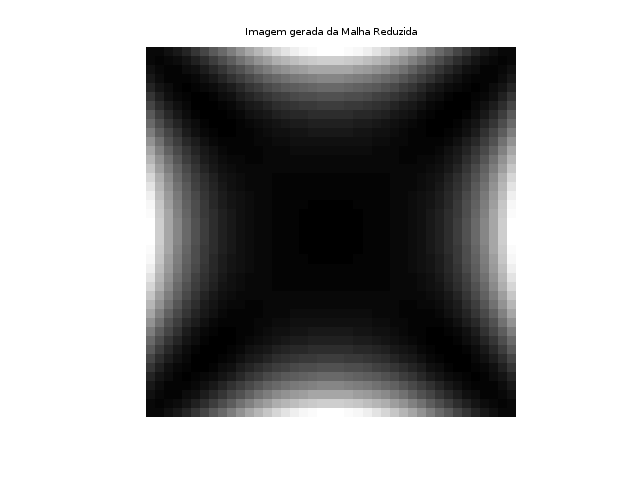
\includegraphics[scale=0.5]{f3_compress_reduced.png}
\caption{Malha interpolada a partir de h(x,y) com o tamanho reduzido}
\end{figure}

\end{document}